\documentclass[nir, och, master]{SCWorks}
%    spec
%    bachelor
%    master
%    och
%    zaoch
%    referat
%    coursework
%    diploma
%    pract
%    pract
%    autoref
%    assignment
%    review
%    critique
%    times
%    nir
\usepackage[T2A]{fontenc}
% \usepackage[cp1251]{inputenc}  %NOTE: uncomment to compile .tex with windows
\usepackage[utf8]{inputenc} %NOTE: comment to compile .tex with windows
\usepackage{graphicx}
% \usepackage[sort,compress]{cite}
\usepackage{amsmath}
\usepackage{amssymb}
\usepackage{amsthm}
\usepackage{fancyvrb}
\usepackage{longtable}
\usepackage{array}
\usepackage[english,russian]{babel}
\usepackage{tempora}
\usepackage[colorlinks=true]{hyperref}


% \usepackage{biblatex}
% \bibliography{thesis} 
% \bibliographystyle{gost2003}  

% \usepackage[
% backend=bibtex,
% %  style=gost2003,
% sorting=ynt
% ]{biblatex}
% \addbibresource{thesis.bib}

% \usepackage[backend=biber,style=ieee]{biblatex}
% \addbibresource{thesis.bib}

\newcommand{\eqdef}{\stackrel {\rm def}{=}}

\newtheorem{lem}{учебная (Научно-исселдовательская работа)}

\begin{document}

\chair{информатики и программирования}
\title{Разработка системы траекторного управления БПЛА}
\course{1}
\group{173}
%\department{}
\napravlenie{02.03.02 "--- Математическое обеспечение и администрирование информационных систем}
\author{Ворониной Екатерины Юрьевны}
\chtitle{доцент кафедры ИиП}
\chname{Е.В. Кудрина}
\satitle{Кандидат ф.-м.наук, доцент}
\saname{М.В. Огнева}
\term{1}
\practtype{учебная ("Научно-исследовательская работа")}
% \duration{2}
\practStart{01.09.2023}
\practFinish{28.12.2023}
\date{2024}

\maketitle

\tableofcontents

\abbreviations
\begin{description}
	\item БПЛА --- беспилотный летательный аппарат;
	\item СТУ --- система траекторного управления;
	\item НПУ --- наземный пункт управления;
	\item АУ --- бортовая аппаратура управления;
	\item НАУ --- наземная аппаратура управления;
	\item БАС --- беспилотная авиационная система;
	\item АПИК --- аналитическая программно-инвариантная конструкция;
	\item СВС --- система воздушных сигналов;
	\item ВПП --- взлетно-посадочная полоса;
	\item БТС --- беспилотная транспортная система;
\end{description}

\intro
Развитие беспилотной авиации входит в область интересов государственной промышленной политики. 
В связи с тем, что  Правительство РФ \cite{rasporyazhenie} утвердило стратегию развития беспилотной авиации до 2030 г. 
и на перспективу до 2035 г., в настоящее время сфера беспилотной авиации получает большую финансовую поддержку со стороны государства.

Нарастающий интерес к беспилотной авиации --- тенденция общемировая. Это происходит по ряду 
причин. БПЛА, как правило, гораздо дешевле пилотируемых самолетов и вертолетов. Дешевле, чем 
подготовка летчика, обходится и подготовка оператора беспилотной системы. Отсутствие пилота 
позволяет исключить бортовые системы жизнеобеспечения, уменьшить массу и габариты БПЛА, 
а также увеличить диапазон допустимых перегрузок и влияющих факторов. Большое значение имеет 
и фактор безопасности — потери беспилотных аппаратов не ведут к потере пилотов.

Взрывной рост количества разработок БПЛА именно в последнее десятилетие не случаен. Этому 
способствовали определенные объективные предпосылки, которые созрели именно к этому времени. 
Они связаны с серьезными технологическими успехами в различных областях. Например, этому 
способствовало \cite{uvDev,kbpa}:
\begin{enumerate}
	\item появление легких и прочных композитных материалов;
	\item развитие микроэлектронной компонентной базы: микроконтроллеров, микросистемных навигационных 
	датчиков, приемопередатчиков радиосигналов, различных СВЧ-устройств, микроэлектронных драйверов 
	сильноточных потребителей, миниатюрных видеокамер и т.д.;
	\item появление и быстрое развитие высокоэффективных возобновляемых источников питания на основе 
	литий-полимерных аккумуляторов, топливных элементов и др.;
	\item разработки в области высокоресурсных бесколлекторных электродвигателей, а также 
	реактивных и поршневых двигателей;
	\item развитие спутниковых систем глобального позиционирования;
	\item общее развитие вычислительной техники, включая появление специальных операционных систем, 
	интерфейсов, математического и алгоритмического обеспечения;
\end{enumerate}


Для управления траекторией движения беспилотного летательного судна решается ряд задач, связанных с планированием и реализацией сложных 
пространственных движений \cite{kbpa}. К этому ряду относится задача нахождения допустимого пути летательного аппарата 
в трехмерном пространстве, огибающего статические препятствия, а также связанные с ней задачи путевой и траекторной  стабилизации. 
Для решения перечисленных задач, необходимо как можно более приближенно оценивать положение и ориентацию БПЛА в режиме реального времени. 
Возрастающая с ростом количества бортовых датчиков сложность системы оценки, а также нарастающая со временем погрешность данных измерений 
бортовых сенсоров приводит к необходиомсти применения алгоритмов: ПИД-регулирования, фильтра Калмана и др.   


Целью данной работы является разработка математической модели БПЛА и анализ подходов к решению задачи системы траекторного управления роторным БПЛА. 
Исходя из цели определены следующие задачи:
\begin{itemize}
	\item обзор видов БПЛА;
	\item определение структуры системы управления БПЛА;
	\item моделирование динамической системы движения БПЛА;
	\item исследование современных подходов к конструкции бортовой системы БПЛА;
	\item анализ алгоритмов обработки данных с бортовых сенсоров;
\end{itemize}
 

\section{Классификация БПЛА}

Летательным аппаратом называется техническое устройство, предназначенное для осуществления полетов в земной 
атмосфере или в космосе \cite{11}. По наличию экипажа все ЛА можно разделить две группы – пилотируемые и беспилотные.

Под термином беспилотный летательный аппарат понимаются ЛА, не имеющие на борту экипажа и способные перемещаться 
в воздухе в автономном режиме, посредством дистанционного управления, оператором с НПУ или сочетанием указанных 
способов \cite{11}. Дистанционное управление БПЛА может осуществляться с помощью дискретных разовых радиокоманд. 
В автономном режиме оператор осуществляет функцию контроля.

В основу классификации БПЛА могут быть положены признаки, характеризующие конструктивные особенности, 
способы управления,  массовые и габаритные параметры. Конструктивно БПЛА разделяются на роторные – с 
вращающимся крылом и самолетные – с неподвижным крылом. На рисунке ~\ref{classification} приведена более подробная классификация БПЛА.

\begin{figure}[!ht]
	\centering
	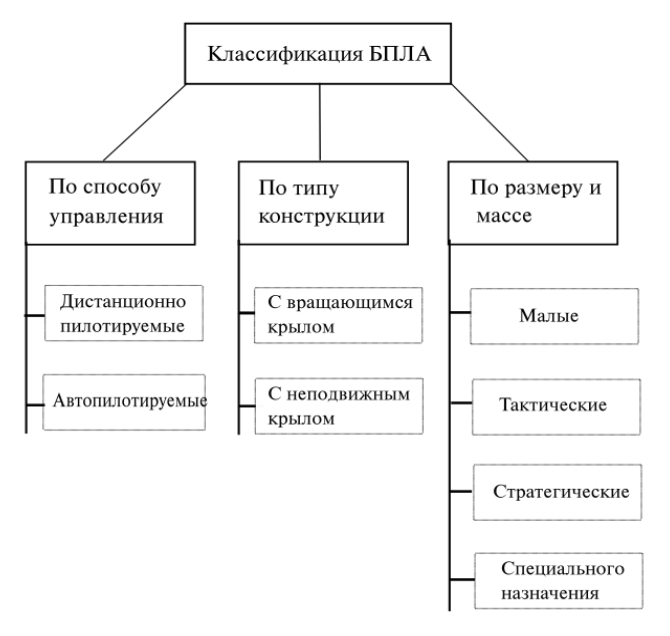
\includegraphics[width=6cm]{img/uav_classification.png}
	\caption{\label{classification}%
	Классификация БПЛА}
\end{figure}

Подъемная сила у БПЛА самолетного типа создается аэродинамическим способом за счет 
напора воздуха, набегающего под неподвижное крыло. Судна самолетного типа, как правило, 
отличаются большей, в сравнении с роторными, длительностью полета, большей максимальной 
высотой полета и высокой скоростью. Но в отличии о роторных моделей, из-за особенностей 
конструкции, самолетные БПЛА не способны зависать в воздухе.

Наиболее распространенным БПЛА является мультикоптер --- роторный БПЛА имеющий больше двух 
несущих винтов \cite{}. Подъемная сила у роторных БПЛА создается силами моментов несущих винтов, 
расположенных параллельно земле. Реактивные моменты уравновешиваются за счет вращения н
есущих винтов попарно в разные стороны или наклона вектора тяги каждого винта в нужном 
направлении.

Квадрокоптер является самой распространенной схемой построения мультикоптеров. 
Квадрокоптер – это четырехроторный БПЛА, способный к вертикальному взлету и посадке, 
который приводится в движение четырьмя несущими винтами, расположенными в одной 
плоскости параллельно земле []. Наличие четырех жестко зафиксированных роторов дает 
возможность организовать довольно простую схему организации движения. Существуют 
две таких схемы движения: схема «+» и схема «х». В первом случае один из роторов 
является передним, противоположный ему – задним, и два ротора являются боковыми. 
В схеме «х» передними являются одновременно два ротора, два других являются задними, 
а смещения в боковом направлении также реализуются одновременно парой соответствующих 
роторов. Алгоритм управления частотами вращения винтов для схемы «+» несколько проще, 
чем для схемы «х», однако последняя используется чаще из-за конструктивных преимуществ: 
при такой схеме проще разместить фюзеляж, который может иметь вытянутую форму, бортовая 
видеокамера имеет более свободный обзор. На рисунке ~\ref{drone} приведена схема направления 
движения винтов квадрокоптера типа схемы «+». В данной работе в качестве управляемой 
конструкции БПЛА выбран квадрокоптер.

\begin{figure}[!ht]
	\centering
	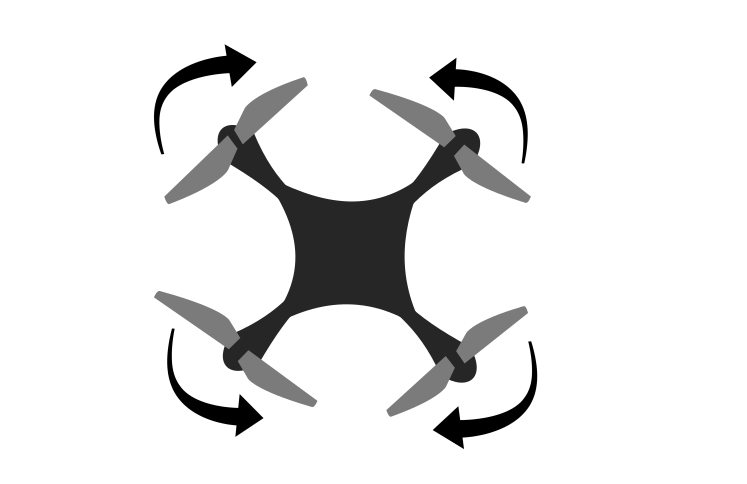
\includegraphics[width=6cm]{img/drone pic.png}
	\caption{\label{drone}%
	Движение винтов квадрокоптера для типа схемы «+»}
\end{figure}


\section{Динамичсекая система движения БПЛА}

\section{Бортовое устройство современных БПЛА}

Основной и самый высокотехнологичный элемент системы БПЛА — это электронная система управления.
Электронная система управления любого БПЛА состоит из вычислительной мощности и сенсоров, включающих в себя:
1. Процессор и/или микроконтроллер с модулями оперативной и энергонезависимой памяти, необходимые
для функционирования систем БПЛА
2. Модуль определения пространственного положения,
состоящий из многоосевых MEMS-сенсоров, таких как
гироскопы, акселерометры, магнетометры и т.д.,
3. Модуль аналоговых или цифровых барометрических
датчиков, для определения высоты
и воздушной скорости,
4. Модуль управления двигателями и энергоснабжением,
5. Модуль управления сервоприводами, для управления
полетом и режимами двигателей
6. Модуль приема спутниковой навигации GPS, для точного геопозиционирования
7. Модуль радиосвязи, для ручного управления и передачи данных телеметрии.
Базовая система управления БПЛА также может дополняться другими системами, такими как радиолокационные системы, лидары, ультразвуковые датчики расстояний, системы стабилизации фото и видеооборудования
и т. д. Данные системы относятся к системам полезной
нагрузки и не являются обязательными и достаточными
для полета БПЛА.

Технология гиростабилизации — компонент дрона,
обеспечивающая плавный полет без рывков. Инерциальный измерительный блок — IMU необходим для отслеживания текущего пространственного положения
БПЛА и предоставления навигационной информации
центральному контроллеру полета. Блок IMU обычно
состоит из гироскопов и акселерометров. Гироскоп
предназначен для определения углов поворота (угловых скоростей) БПЛА. Акселерометр предназначен
для измерения ускорения устройства и корректировки
гироскопов. Некоторые инерциальные измерительные блоки включают в себя магнитометр (компас) для
дополнительной стабилизации БПЛА и определения
направления полета (курса).
Технология геопозиционирования (GPS) совмещенная с внутренним компасом позволяют беспилотному летательному аппарату и системе дистанционного
управления определять местоположение дрона в полёте. Исходная точка взлета, определенная системой
геопозиционирования, задается как место, в которое
дрон приземлится в случае отсутствия сигнала между
ним и системой дистанционного управления (Failsafe
point). Для того чтобы повысить безопасность полетов
и предотвратить случайные полеты в запрещенных зонах, последние модели дронов включают функцию «No
Fly Zone» — «Бесполетная зона».

Технология управления БПЛА реализуется при помощи пульта дистанционного управления или посредством приложения для смартфона. Приложение для
мобильных устройств предоставляет полный контроль
над дроном. Система управления полётом обменивается данными с приемником сигналов, установленным
на ПК, через разъем USB. Это позволяет настраивать
беспилотный летательный аппарат и обновлять прошивку БПЛА. В большинстве дронов встроен контроллер наземной станции или приложение, которое отслеживает текущую телеметрию полёта и «видит»
на мобильном устройстве то, что «видит» дрон.

Для обозначения углов, характеризующих положение БПЛА в пространстве во время полета, 
используются следующие термины: крен, тангаж и рыскание \cite{11}. 
На рисунке \ref{drone_position}

\begin{figure}[!ht]
	\centering
	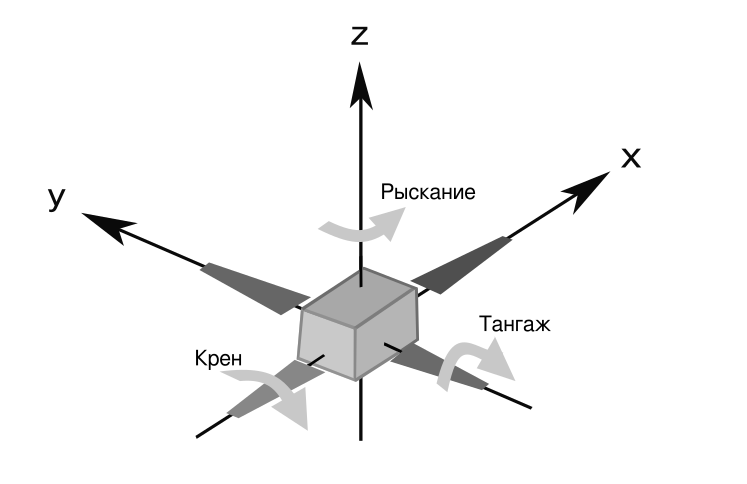
\includegraphics[width=6cm]{img/Navigate SCHEME.png}
	\caption{\label{drone_position}%
	Характеристики движения ЛА в пространстве}
\end{figure}

Крен – отклонение плоскости симметрии ЛА от вертикального положения. 
Характеризуется углом крена и скоростью крена. Манёвры крена используются, 
например, при разворотах, при выполнении фигур пилотажа, при заходе на посадку 
для парирования, смещения траектории летательного аппарата относительно оси 
взлётно-посадочной полосы [11]. Управление креном БПЛА самолетного типа 
осуществляется элеронами – элементами механизации крыла. Управление креном 
роторных БПЛА осуществляются путем изменением скорости вращения одного или 
двух винтов. Повышение оборотов на роторах с левой  стороны квадрокоптера 
вызывает крен и заставляет лететь его в правую сторону. Разворот роторного 
БПЛА вокруг своей оси осуществляется путем увеличения скорости оборотов 
одной симметричной пары винтов, и в равной мере уменьшением оборотов у 
другой пары, нескомпенсированный реактивный момент вызовет вращение машины 
вокруг своей вертикальной оси. Более подробно механизм движения квадрокоптера 
изображен на рисунке \ref{drone_run}.

\begin{figure}[!ht]
	\centering
	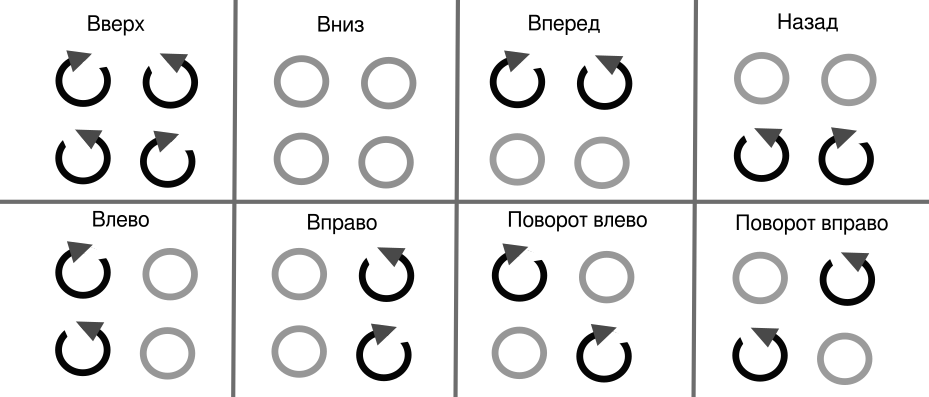
\includegraphics[width=6cm]{img/uavRun.png}
	\caption{\label{drone_run}%
	Механизм движения квадрокоптера}
\end{figure}

Тангаж – угловое движение ЛА, при котором его продольная ось изменяет свое 
направление относительно горизонтальной плоскости. Характеризуется углом тангажа 
и скоростью тангажа. Маневры авиамодели с увеличением угла тангажа называются 
кабрированием, а с уменьшением – пикированием. Эти манёвры  для моделей самолетного 
типа осуществляются созданием момента тангажа за счет отклонения органов управления: 
руля высоты или элевонов. Маневры роторных БПЛА осуществляются путем изменения 
скорости вращения одного или двух винтов.

Рыскание – угловые движения ЛА вокруг вертикальной оси.

Для вычисления траектории полета ЛА, на борту БПЛА устанавливаются разного рода 
измерительные датчики [10, 11], образующие в совокупности со специальным 
ПО-обработчиком систему воздушных сигналов.

Система воздушных сигналов (СВС) БПЛА представляет собой программно-аппаратную 
систему, предназначенную для измерения, вычисления и выдачи на индикацию в 
бортовые системы информации о температуре воздуха, скорости и высоте полета 
летательного аппарата [].

Далее по группам назначения перечислены бортовые измерительные приборы, 
используемые в системе СВС.

\subsection*{Измерение высоты}

Барометрический высотомер – прибор для измерения давления атмосферного воздуха. 
Изменение атмосферного давления связано с изменением высоты полета – давление 
атмосферного воздуха уменьшается с увеличением высоты над уровнем моря [12]. (https://base.garant.ru/187535/81e3ca2c03664592faeb003808d05cd8/)

Барометрической высотой называется высота полета, измеряемая относительно 
изобарической поверхности атмосферного давления, установленного на шкале 
барометрического высотомера. Барометрическая высота может быть 
[https://x-airways.ru/va/modules/wiwimod/index.php?page=%D0%A7%D1%82%D0%BE+%D1%82%D0%B0%D0%BA%D0%BE%D0%B5+QNH,+QFE,+QNE?+%D0%94%D0%B0%D0%B2%D0%BB%D0%B5%D0%BD%D0%B8%D0%B5,+%D0%B2%D1%8B%D1%81%D0%BE%D1%82%D1%8B,+%D1%8D%D1%88%D0%B5%D0%BB%D0%BE%D0%BD%D1%8B.&back=%D0%A1%D0%BE%D0%B4%D0%B5%D1%80%D0%B6%D0%B0%D0%BD%D0%B8%D0%B5]:
\begin{enumerate}
	\item Относительной, если она измеряется относительно давления аэродрома вылета или посадки. 
	Используется при полетах ниже нижнего эшелона в зоне взлета и посадки;
	\item Приведенной, если она измеряется относительно минимального давления участка трассы, 
	которое приведено к уровню моря. Используется при визуальных полетах по маршруту ниже 
	нижнего эшелона;
	\item Условно барометрической, если она измеряется относительно стандартного уровня давления 
	760 мм.рт.ст. (1013 ГПа, 29,92 д.рт.ст.). Используется для выдерживания заданных эшелонов 
	при полетах по трассам и в зоне ожидания;
\end{enumerate}
 
Применительно к первым двум значениям используется термин высота. А когда речь идет о 
третьем пункте – говорят про эшелон.

В момент, когда перед взлетом воздушное судно выруливает на ВПП, на высотомерах 
устанавливается давление аэродрома вылета, высотомеры  показывают ноль. 
После взлета на высотомерах устанавливается давление 760 мм.рт.ст и 
набирается заданный эшелон. На снижении на высотомерах устанавливается 
давление аэродрома посадки, и после приземления высотомеры снова показывают ноль.

Высота перехода – установленная в районе аэродрома высота для перевода шкалы 
давления барометрического высотомера на значение давления 760 мм.рт.ст. (1013,2 мБар) 
при наборе заданного эшелона.

Радиовысотомер – измеряет время прохождения радиосигнала от антенны на 
воздушном судне до поверхности и в обратную сторону. Конструктивно прибор 
состоит из СВЧ-радиопередатчика, антенна которого обычно располагается в 
нижней части судна, приемника сигналов и системы их обработки и вывода в кабину, 
а также сигнализации при угрозе столкновения с землей.

\subsection*{Измерение скорости}
Датчики статического(барометр) и полного давлений и датчики температуры наружного воздуха применяются для определения скоростного напора, числа Маха и воздушной приборной скоростей. 
уравнение Бернулли.
Подъемная сила, действующая на самолет равна Y = ½CYSρV2


\subsection*{Измерение ускорений}
Гироскоп – навигационный прибор, основным элементом которого является быстро 
вращающийся ротор, закрепленный так, что ось его вращения может поворачиваться. 
Если поворот оси гироскопа ограничить пружиной, то при установке его на 
летательном аппарате, во время выполнения ЛА разворота, гироскоп будет 
деформировать пружину, пока не уравновесится момент внешней силы. 
В этом случае сила сжатия или растяжения пружины пропорциональна угловой скорости 
движения летательного аппарата. Таков принцип действия авиационного 
указателя поворота и многих других гироскопических приборов.

Акселерометр – прибор, измеряющий проекцию кажущегося ускорения. 
Как правило, акселерометр представляет собой чувствительную массу, 
закрепленную в упругом подвесе. Отклонение массы от ее первоначального 
положения при наличии кажущегося ускорения несёт информацию о величине этого ускорения. 

\subsection*{Измерение углов крена и тангажа}
Пирометр – оптический прибор, измеряющий температуру тел без непосредственного 
контакта. В авиации используется устройство пирогоризонт, состоящее из из двух 
пар пирометрических датчиков, расположенных под углом 90 градусов. 
Если модель летит горизонтально, каждый датчик «видит» 50\%
небосвода и 50\% земли. Показания диаметрально противоположных датчиков равны, то есть: 

$Dat_1 – Dat_3 = 0,

Dat_2 – Dat_4 = 0$

Для вычисления углов крена и тангажа необходимо знать рассогласование, 
возникающее, когда датчики видят 100\% неба и 100\% земли. Для этого необходимо 
на земле, перед вылетом, разместить модель вертикально по крену и тангажу, и 
зафиксировать показания  датчиков в этих положениях. Тогда углы крена и тангажа 
могут быть вычислены по формулам [13, 14]: 

$\gamma = \dfrac{(D_1 - D_3) * 90 }{D_1 - D_3}, \\ \theta = \dfrac{(D_2 - D_4) * 90}{D_2 - D_4}$, где \\
$D_x, x \in [0, 4]$ --- показатель соответсвующего пиродатчика.
$\gamma$ --- угол крена.
$\theta$ --- угол тангажа.

Линия на поверхности Земли, разделяющая зону видимости радиолокатора и его «слепую» зону, 
называется радиолокационным горизонтом [14].

Датчики статического и полного давлений и датчики температуры наружного воздуха применяются 
для определения высоты полета, скоростного напора, числа Маха и воздушной приборной скоростей.

Скоростной напор  – . Полное давление = динамическое давление (скоростной напор) + статическое давление.

Воздушная приборная скорость –

Число Маха – основная характеристика течения газа, равная отношению скорости течения к скорости звука 
в той же точке потока: 

$М = \dfrac{v}{a}$, где 
$v$ --- скорость ЛА.

$a$ --- скорость звука.
 
Число Маха является одним из основных критериев аэродинамического подобия для случаев, 
когда нельзя пренебрегать сжимаемостью газа. В воздухе сжимаемость необходимо 
учитывать при $v > 100$ м/сек, которым соответствует $М > 0,3$. При $М < 1$ 
течение называется дозвуковым, при $М = 1$ — звуковым, а при $М > 1$ — сверхзвуковым. 
Одна из основных особенностей сверхзвуковых течений — образование ударных волн при обтекании 
тел или торможении потока газа. В результате диссипации энергии в ударных волнах возникает 
волновое сопротивление, величина которого увеличивается с ростом числа Маха.


\subsection*{Навигация}

GPS

\subsection*{Подъемная сила}

Коллекторные двигатели – 
Бесколлекторные двигатели –
Электронный регулятор скорости (ESC) – это электронная схема, установленная на каждом 
двигателе и предназначенная для изменения оборотов электродвигателя, его направления, 
а также торможения.

Бесколлекторный двигатель постоянного тока используются исключительно в квадрокоптерах, 
поскольку их тяга выше, чем у коллекторных двигателей постоянного тока. Коммутаторы в 
бесколлекторных двигателях встроены в регулятор скорости, в то время как коллекторы 
щеточных двигателей постоянного тока расположены непосредственно внутри двигателя. 
Бесколлекторные двигатели имеют лучшие характеристики скорости и крутящего момента, 
высокую эффективность, бесшумно работают, имеют очень высокий диапазон оборотов, 
имеют более длительный срок службы.

Литий-полимерные (LiPo) аккумуляторные батареи массово используются для питания квадрокоптеров, 
поскольку они обладают высокой удельной энергией и малым весом. Аккумулятор используется 
для питания двигателей и всех электронных компонентов квадрокоптера.



\section{Программно-алгоритмического обеспечения САУ БПЛА}

Дроны оснащены встроенным программным обеспечением, которое отправляет команды исполняющим
устройствам БПЛА или удалённому контроллеру.
Во многом качество и надежность системы управления БПЛА зависит от программного обеспечения.
В последние годы для управления роботизированными системами, в том числе и БПЛА, широкое распространение получили операционные системы реального времени (ОСРВ). Такие операционные системы
позволяют реагировать БПЛА на возникающие события и изменения в окружающей обстановке с высокой скоростью. Применение ОСРВ позволяет полностью
автоматизировать функционирование БПЛА, оператор
в данном случае лишь задает полетное задание и выполняет задачи, не связанные с контролем за полетом,
например, производит аэрофотосъемку, топографическую съемку и т.д.


Устройство стандартного дрона вертолетного типа
(квадрокоптер) и основные узлы БПЛА представлены
на рисунке 

Как видно из приведенной схемы отличие различных
типов дронов заключается в аэродинамической схеме
(вертолетный, самолетный типы, БПЛА вертикального
взлета и посадки и т.п.). Электронно-механические системы управления как правило различаются не значительно и только в части полезной нагрузки (дополнительного оборудования)

ПОЛЕЗНАЯ НАГРУЗКА БПЛА
Лидарные, мультиспектральные и фотограмметрические датчики используются для создания трёхмерных
моделей зданий и ландшафтов. Датчики ночного видения используются для работы при слабом освещении,
тепловизионные датчики используются для сканирования зданий и ландшафтов, оказания помощи в сельском хозяйстве, пожаротушении, поисковых и спасательных операциях.
Беспилотниками управляют с помощью систем дистанционного управления с земли. Беспилотный летательный аппарат состоит: из самого дрона и системы
управления.
Дроны оснащают системами предотвращения столкновений. В системе искусственного зрения применяются датчики обнаружения препятствий для сканирования окружающей среды, вместе с тем, программные
алгоритмы и технология SLAM переносят изображения
в трёхмерные карты, позволяя контроллеру полёта обнаруживать препятствия и избегать столкновения
с ними. Эти системы объединяют один или несколько
датчиков для обнаружения и обхода препятствий:
• датчик изображения;
• ультразвуковой датчик;
• инфракрасный датчик;
• лидар;
• инерциальные навигационные модули;
• монокулярное зрение.

БТС представляет собой не  одну технологию, а сложную систему технологий, состоящую из 
множества подсистем. Итак, разобьем их на три основные группы \cite{китайцв}: 
\begin{enumerate}
	\item алгоритмы сенсорного сканирования, восприятия и принятия решений 
	(требующие, как правило, построения сложных логических выводов); 
	\item клиентские системы, включая операционную систему и аппаратную платформу;
	\item облачные платформы, в том числе создание карт высокой четкости (HD-карт), 
	обучение моделей глубокого обучения, моделирование и хранение данных;
\end{enumerate}

Hight Definition (HD) maps — карты с точным месторасположением объектов в векторном формате. 
Они содержат детали, которых нет на обычных картах: знаки, светофоры, разметку, столбы, 
даже кусты, если это необходимо для навигации.

Первая подсистема отвечает за извлечение важной информации из необработанных данных, 
полученных сенсорами, и обеспечивает исследование роботом окружающей среды, на чем в 
дальнейшем строится принятие решений относительно его будущих действий. Клиентские системы 
объединяют алгоритмы первой подсистемы, тем самым позволяя им работать в режиме реального
времени и обеспечивая надежность. Например, если камера генерирует данные
с частотой 60 Гц, клиентским системам необходимо убедиться, что самый длинный этап 
обработки занимает менее 16 мс. Платформа облачных вычислений отвечает за автономные 
вычисления и хранение данных. С ее помощью мы можем тестировать новые алгоритмы, 
обновлять HD-карты и обучать БТС более качественным моделям распознавания, 
отслеживания и принятия решений.
  


% \begin{equation}
% 	F(x)=\int\limits_a^bf(x)\,dx.
% \end{equation}

% testtesttesttesttesttest testtest testtesttesttesttesttesttest~\ref{fig:f}.
% \begin{figure}[!ht]
% 	\centering
% 	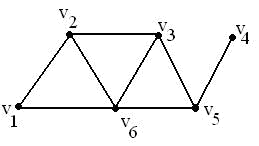
\includegraphics[width=6cm]{fig2.png}
% 	\caption{\label{fig:f}%
% 	testtesttesttesttesttesttest test testtesttesttesttesttesttest}
% \end{figure}



% \begin{figure}[ht]
% 	\centering
% 	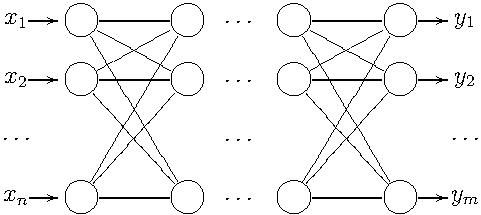
\includegraphics{NN-Scheme}
% 	\caption{testtesttesttesttesttesttesttesttesttesttest testtesttesttesttesttesttesttesttesttesttesttest testtesttesttest testtesttesttesttesttesttest
% 	testtesttesttesttesttesttesttesttesttesttesttesttesttesttest}\label{net1}
% \end{figure}

% \begin{table}[!ht]
% 	\small
% 	\caption{что то } \label{table-1}
% 	\begin{tabular}{|l|c|c|c|c|r|r|r|}
% 		\hline 1 & 2& 3& 4& 5& 6& 7& 8\\
% 		\hline S298 & 177 & 1932 & 341964 & 61 & 10797 & 3,16\% & 0,61\\
% 		\hline S344 & 240 & 1397 & 335280 & 59 & 14160 & 4,22\% & 0,53\\
% 		\hline S349 & 243 & 1474 & 358182 & 62 & 15066 & 4,21\% & 0,60\\
% 		\hline S382 & 190 & 12444 & 2364360 & 55 & 10450 & 0,44\% & 3,78\\
% 		\hline S386 & 274 & 2002 & 548548 & 91 & 24934 & 4,55\% & 1,40\\
% 		\hline S400 & 194 & 13284 & 2577096 & 58 & 11252 & 0,44\% & 4,28\\
% 		\hline S444 & 191 & 13440 & 2567040 & 60 & 11460 & 0,45\% & 4,26\\
% 		\hline S510 & 446 & 700 & 312200 & 70 & 31220 & 10,00\% & 0,63\\
% 		\hline S526 & 138 & 13548 & 1869624 & 38 & 5244 & 0,28\% & 2,41\\
% 		\hline S641 & 345 & 5016 & 1730520 & 132 & 45540 & 2,63\% & 7,06\\
% 		\hline S713 & 343 & 3979 & 1364797 & 131 & 44933 & 3,29\% & 5,61\\
% 		\hline S820 & 712 & 21185 & 15083720 & 244 & 173728 & 1,15\% & 126,99\\
% 		\hline S832 & 719 & 21603 & 15532557 & 253 & 181907 & 1,17\% & 135,18\\
% 		\hline S953 & 326 & 322 & 104972 & 91 & 29666 & 28,26\% & 0,27\\
% 		\hline S1423 & 293 & 750 & 219750 & 93 & 27249 & 12,40\% & 0,57\\
% 		\hline S1488 & 1359 & 22230 & 30210570 & 384 & 521856 & 1,73\% & 541,69\\
% 		\hline
% 	\end{tabular}
% \end{table}


% testtesttest testtesttesttesttesttesttest testtesttesttesttesttesttesttesttesttest testtesttesttesttesttesttesttesttest testtesttesttesttesttesttest:
% \[
%     \left(
%     \begin{matrix}
%         1 & 0 & 5 & 0 & 0 \\
%         0 & 2 & 7 & 4 & 0 \\
%         0 & 0 & 1 & 0 & 0 \\
%         9 & 6 & 0 & 3 & 0 \\
%         0 & 0 & 3 & 0 & 5
%     \end{matrix}
%     \right)
% \]


\conclusion
В ходе работы было выполнено:
\begin{itemize}
    \item это
    \item и это
\end{itemize}

% \printbibliography[title = Reference List]

 

\appendix

\section{test}

\begin{table}[!ht]
	\footnotesize
	\caption{Results of pass-fail dictionary reduction with the help
	of masks} \label{table-2}
	\begin{tabular}{|p{1.5cm}|
	                 p{1.5cm}|
	                 p{1.5cm}|
	                 p{1.5cm}|
	                 p{1cm}|
	                 p{1.5cm}|
	                 p{1.5cm}|
	                 p{1cm}|}
		\hline \centering Circuit & Number of modelled faults & Number of test
		vectors in the test set & The volume of pass-fail dictionary,
		\linebreak bit & The volume of found mask & The volume of
		masked dictionary, \linebreak bit & \raggedright \% of pass-fail dictionary
		& CPU running time, \linebreak min
		\\
		\hline S298 & 177 & 322 & 56994 & 30 & 5310 & 9,32\% & 0,07\\
		\hline S344 & 240 & 127 & 30480 & 29 & 6960 & 22,83\% & 0,04\\
		\hline S349 & 243 & 134 & 32562 & 35 & 8505 & 26,12\% & 0,05\\
		\hline S382 & 190 & 2074 & 394060 & 28 & 5320 & 1,35\% & 0,43\\
		\hline S386 & 274 & 286 & 78364 & 65 & 17810 & 22,73\% & 0,26\\
		\hline S400 & 194 & 2214 & 429516 & 32 & 6208 & 1,45\% & 0,99\\
		\hline S444 & 191 & 2240 & 427840 & 30 & 5730 & 1,34\% & 0,98\\
		\hline S526 & 138 & 2258 & 311604 & 28 & 3864 & 1,24\% & 0,61\\
		\hline S641 & 345 & 209 & 72105 & 58 & 20010 & 27,75\% & 0,24\\
		\hline S713 & 343 & 173 & 59339 & 58 & 19894 & 33,53\% & 0,19\\
		\hline S820 & 712 & 1115 & 793880 & 147 & 104664 & 13,18\% & 9,09\\
		\hline S832 & 719 & 1137 & 817503 & 151 & 108569 & 13,28\% & 9,20\\
		\hline S953 & 326 & 14 & 4564 & 13 & 4238 & 92,86\% & 0,01\\
		\hline S1423 & 293 & 150 & 43950 & 58 & 16994 & 38,67\% & 0,15\\
		\hline S1488 & 1359 & 1170 & 1590030 & 158 & 214722 & 13,50\% & 26,69\\
		\hline
	\end{tabular}
\end{table}

\begin{equation}
  F(x)=\int\limits_a^bf(x)\,dx.
\end{equation}


\begin{figure}[!ht]
	\centering
	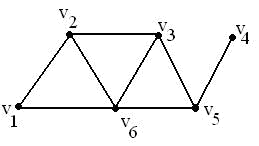
\includegraphics[width=6cm]{fig2.png}
	\caption{\label{fig:f3}%
	test}
\end{figure}


\begin{table}[!ht]
\caption{}
\begin{tabular}{|c|c|}
  \hline
  0 & 1\cr
  \hline
  1 & 0\cr
  \hline
\end{tabular}
\end{table} 


\bibliographystyle{gost780uv} % стиль цитат
\bibliography{thesis} % вместо bibliography нужно указать название вашего .bib файла без расширения (т.е. тут будет использован файл "bibliography.bib")

\end{document}
